\documentclass[12pt, a4paper]{article}
\usepackage[utf8]{inputenc}
\usepackage{physics}
\usepackage{graphicx}
\usepackage{amsmath}
\usepackage{cancel}

\usepackage{MnSymbol}%
\usepackage{wasysym}%
%code color
\usepackage{listings}
\usepackage{xcolor}

\definecolor{codegreen}{rgb}{0,0.6,0}
\definecolor{codegray}{rgb}{0.5,0.5,0.5}
\definecolor{codepurple}{rgb}{0.58,0,0.82}
\definecolor{backcolour}{rgb}{0.95,0.95,0.92}

\lstdefinestyle{mystyle}{
	backgroundcolor=\color{backcolour},   
	commentstyle=\color{codegreen},
	keywordstyle=\color{magenta},
	numberstyle=\tiny\color{codegray},
	stringstyle=\color{codepurple},
	basicstyle=\ttfamily\footnotesize,
	breakatwhitespace=false,         
	breaklines=true,                 
	captionpos=b,                    
	keepspaces=true,                 
	numbers=left,                    
	numbersep=5pt,                  
	showspaces=false,                
	showstringspaces=false,
	showtabs=false,                  
	tabsize=2
}

\lstset{style=mystyle}

\begin{document}
	Mr. Phiphat Chomchit 630631028
	\begin{center}
		\textbf{Test 7: Quantum Teleportation (10/17/2021) }
			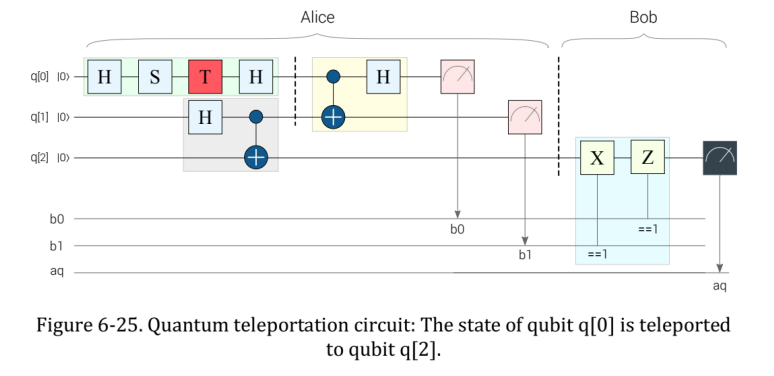
\includegraphics[scale=0.7]{problem.png}
	\end{center}

	\newpage
	
	\begin{enumerate}
		\item Quantum Teleportation Circuit.
		\begin{lstlisting}[language=Python, caption= Circuit]
			from qiskit import QuantumRegister, ClassicalRegister, QuantumCircuit
			qreg_q = QuantumRegister(3, 'q')
			creg_b0 = ClassicalRegister(1, 'b0')
			creg_b1 = ClassicalRegister(1, 'b1')
			creg_aq = ClassicalRegister(1, 'aq')
			circuit = QuantumCircuit(qreg_q, creg_b0, creg_b1, creg_aq)
			
			circuit.h(qreg_q[0])
			circuit.s(qreg_q[0])
			circuit.t(qreg_q[0])
			circuit.h(qreg_q[0])
			circuit.h(qreg_q[1])
			circuit.cx(qreg_q[1], qreg_q[2])
			
			circuit.barrier(qreg_q[0], qreg_q[1])
			circuit.cx(qreg_q[0], qreg_q[1])
			circuit.h(qreg_q[0])
			circuit.measure(qreg_q[0], creg_b0[0])
			circuit.measure(qreg_q[1], creg_b1[0])
			circuit.barrier(qreg_q[0], qreg_q[1], qreg_q[2])
			
			circuit.x(qreg_q[2]).c_if(creg_b1, 1)
			circuit.z(qreg_q[2]).c_if(creg_b0, 1)
			circuit.measure(qreg_q[2], creg_aq[0])
			
			#drawing the circuit
			circuit.draw('mpl')
			
		\end{lstlisting}
		
		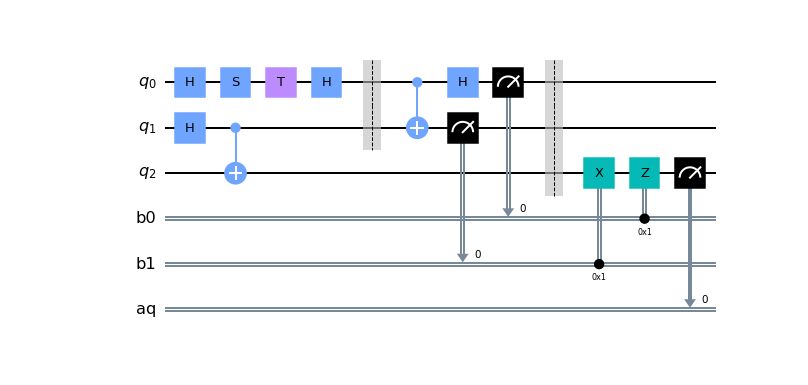
\includegraphics[scale=0.4]{circuit.png}
		
		\item Simulation and Visualization of the Result.
		\begin{lstlisting}[language=Python, caption= Simulation and Visualization]
			# Adding the transpiler to reduce the circuit to QASM instructions
			# supported by the backend
			from qiskit import transpile
			
			# Use Aer's qasm_simulator
			from qiskit.providers.aer import QasmSimulator
			
			backend = QasmSimulator()
			
			# First we have to transpile the quantum circuit
			# to the low-level QASM instructions used by the
			# backend
			qc_compiled = transpile(circuit, backend)
			
			# Execute the circuit on the qasm simulator.
			# We've set the number of repeats of the circuit
			# to be 1024, which is the default.
			job_sim = backend.run(qc_compiled, shots=1024)
			
			# Grab the results from the job.
			result_sim = job_sim.result()
			
			from qiskit.visualization import plot_histogram
			plot_histogram(counts)
		\end{lstlisting}
		\begin{center}
			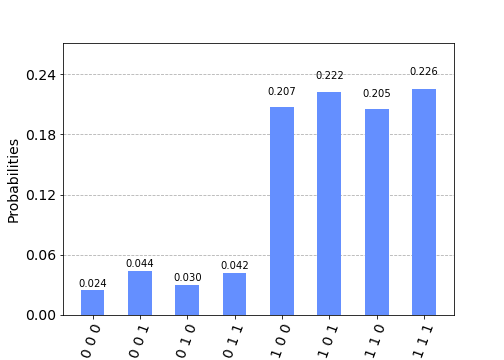
\includegraphics[scale=0.5]{hist.png}
		\end{center}
		
	
	\end{enumerate}
\end{document}
